\documentclass{article}
\usepackage[utf8]{inputenc}
\usepackage{geometry}
\usepackage{fancyhdr}
\usepackage[pdftex]{graphicx}
\usepackage{cite}
\usepackage{listings}
\usepackage{caption}
\usepackage{color}
\usepackage{underscore}
\usepackage{url}

  \usepackage{courier}

% from http://stackoverflow.com/questions/741985/latex-source-code-listing-like-in-professional-books
 \lstset{
         basicstyle=\footnotesize\ttfamily, % Standardschrift
         numbers=left,               % Ort der Zeilennummern
         numberstyle=\tiny,          % Stil der Zeilennummern
         %stepnumber=2,               % Abstand zwischen den Zeilennummern
         numbersep=5pt,              % Abstand der Nummern zum Text
         tabsize=2,                  % Groesse von Tabs
         extendedchars=true,         %
         breaklines=true,            % Zeilen werden Umgebrochen
         keywordstyle=\color{red},
            frame=b,         
%        keywordstyle=[1]\textbf,    % Stil der Keywords
%        keywordstyle=[2]\textbf,    %
%        keywordstyle=[3]\textbf,    %
%        keywordstyle=[4]\textbf,   \sqrt{\sqrt{}} %
         stringstyle=\color{white}\ttfamily, % Farbe der String
         showspaces=false,           % Leerzeichen anzeigen ?
         showtabs=false,             % Tabs anzeigen ?
         xleftmargin=17pt,
         framexleftmargin=17pt,
         framexrightmargin=5pt,
         framexbottommargin=4pt,
%         showstringspaces=false      % Leerzeichen in Strings anzeigen ?        
 }

\DeclareCaptionFont{white}{ \color{white} }
\DeclareCaptionFormat{listing}{
  \colorbox[cmyk]{0.43, 0.35, 0.35,0.01 }{
    \parbox{\textwidth}{\hspace{15pt}#1#2#3}
  }
}
\captionsetup[lstlisting]{ format=listing, labelfont=white, textfont=white, singlelinecheck=false, margin=0pt, font={bf,footnotesize} }

%TCIDATA{OutputFilter=LATEX.DLL}
%TCIDATA{Version=5.50.0.2953}
%TCIDATA{<META NAME="SaveForMode" CONTENT="1">}
%TCIDATA{BibliographyScheme=Manual}
%TCIDATA{Created=Monday, January 30, 2012 17:20:46}
%TCIDATA{LastRevised=Monday, February 27, 2012 12:06:08}
%TCIDATA{<META NAME="GraphicsSave" CONTENT="32">}
%TCIDATA{<META NAME="DocumentShell" CONTENT="Standard LaTeX\Blank - Standard LaTeX Article">}
%TCIDATA{CSTFile=40 LaTeX article.cst}

\newenvironment{proof}[1][Proof]{\noindent\textbf{#1.} }{\ \rule{0.5em}{0.5em}}

% Sets page margins to 1", which is standard
\geometry{left=1in,right=1in,top=1in,bottom=1in} 

% allows the included extensions of graphic files
\DeclareGraphicsExtensions{.pdf,.png,.jpg}

% sets/adds graphic path. If empty it just looks around the folder the .tex file is in
\graphicspath{{}}

% I do not remember what this does
\setlength{\headheight}{15.2pt}

% allows the xhead parameters
\pagestyle{fancy}

% Sets the left header
\lhead{Group Awesome}

% Sets the right header
\rhead{Exercise 1, TDT4255 Autumn 2013}

% everything before this is considered the header or whatever.
\begin{document}

% INCLUDEGRAPHICS EXPLANATION
% \includegraphics[scale=1]{name of file}
% sometimes you want to twice encase the filename in squiggly brackets. I do not know why but sometimes it is required.

% begin title page, use \\ for newline
\title{Report from exercise \#1\\TDT4255 Computer Design}

% now one can list the authors, \textbf{} makes bold text
\author{Emil Taylor Bye \and Péter Henrik Gombos \and Per Thomas Lundal}


\pagenumbering{roman}

% make title page
\maketitle


\bigskip
\bigskip
\bigskip
\bigskip

\part*{Abstract}

In this report we will describe our implementation of a Simple Multi-Cycle MIPS processor in VHDL. We will describe the motivation, technical details of the implementation and our process.


\newpage

\tableofcontents

\setcounter{secnumdepth}{3}

\newpage

\setcounter{page}{1}
\pagenumbering{arabic}

\part{Introduction}

\section{Processor design and VHDL}
In processor design, thousands of transistors have to be carefully arranged.
Every single connection can make or break the design, thus manual placement and
wiring is obviously no option.  However through the use of Hardware Description
Languages (HDL), designers can specify the semantics of their circuits through a
programming-like syntax, and allow a software tool to synthesize the HDL code
into a low-level schematic of the circuit, greatly simplifying the process and
improving efficiency.


VHDL is one such language.  It was originally developed at the hands of the U.S
Department Of Defense to document the behavior of Integrated Circuits (ICs), but
was later expanded to allow logic simulation and synthesis. The language is
documented in the IEEE Standard 1076, and the last revision was added in
2008.\cite{ieee-1076}

VHDL is used not only to synthesize hardware design, but as it's a complete
programming language, it is used for simulation of test benches as well. When
writing code that is to be synthesized this must be accounted for, as normal
programming paradigms will make the code unsynthesizable.


\section{FPGA}
Field-Programmable Gate Arrays (FPGAs) are ICs where the logic design can be
reconfigured after manufacturing.  They mainly consists of Look-Up tables
(LUTs), which can be implement any logical expressions, and configurable wiring.
Many also contains Block RAM (BRAM) and hardware accelerators in the form of
adder/subtractors, multipliers and more.  Although FPGAs are not comparable to
Application-Specific ICs (ASICs) in raw performance, they allow for quick and
easy testing and remediation of errors, in addition to being cheaper by far due
to mass-production.


\section{MIPS}
MIPS (acronym for Multiprocessor without Interlocked Pipeline Stage), is a RISC
architecture. The instructions are all coded as 32 bit words, with a small
number of different formats, R, I and J (for register, immediate and jump). 

\begin{figure}[ht]
    \centering
    \begin{tabular}{ | c | c | c | c | c | c | }
        \hline
        op & rs & rt & rd & shamt & func \\
        \hline
    \end{tabular}
    \caption{\label{fig:rInstruction}Instruction format of R-instruction}
\end{figure}

The R-instruction takes three registers, and is used like the following code
snippet:

\begin{verbatim}
    rs = rt + rd
\end{verbatim}

The plus is just for reading convenience, and can be exchanged with a different
opcode and/or func value. The shamt field tells how many positions to shift,
when used with a shift function.

\begin{figure}[ht]
    \centering
    \begin{tabular}{ | c | c | c |  c  | }
        \hline
        op & rs & rt & constant or address   \\
        \hline
    \end{tabular}
    \caption{\label{fig:iInstruction}Instruction format of I-instruction}
\end{figure}

The immediate instruction is used for immediate arithmetic and load/store
instructions, as well as branching. 


\begin{figure}[ht]
    \centering
    \begin{tabular}{ | c | c c c c c c c c c | }
        \hline
        op & & & & & address & & & &  \\
        \hline
    \end{tabular}
    \caption{\label{fig:jInstruction}Instruction format of J-instruction}
\end{figure}

The J-instruction is used for unconditional jumps.


Sources:

MIPS-lecture (\#3)


\newpage

\part{Description}

The assignment was to design a simple multi-cycle processor in VHDL.
It should then be synthesized and simulated using the logic simulation tool ModelSim[TODO ref].
Finally the design should be run and tested on the FPGA onboard a MicroBlaze-based embedded system.

\section{Instruction set}
The processor was required to follow the MIPS instruction set,
where atleast the following instructions was needed to be implemented.
\begin{itemize}
    \item Several ALU instructions (All working on two registers and storing the result in a third):
        \begin{itemize}
            \item ADD - Addition
            \item SUB - Subtraction
            \item SLT - Test if the first source register is less than second
            \item AND - Bitwise and
            \item OR  - Logical or
        \end{itemize}
    \item BEQ - branch if registers are equal
    \item LW - Load word from memory
    \item SW - Store word to memory
    \item LUI - Store immediate value shifted left 16 bits in a register
    \item J - Jump
\end{itemize}

\section{Supplied Materials}
We were given various support material:
\begin{itemize}
    \item Suggested MIPS Architecture - See figure \ref{fig:sugarchi}
    \item Communication Framework - Providing an interface towards the embedded system
    \item VHDL Components - Register File, ALU and Adder
    \item Test Program - For verification of design
\end{itemize}

\begin{figure}[ht]
    \centering
    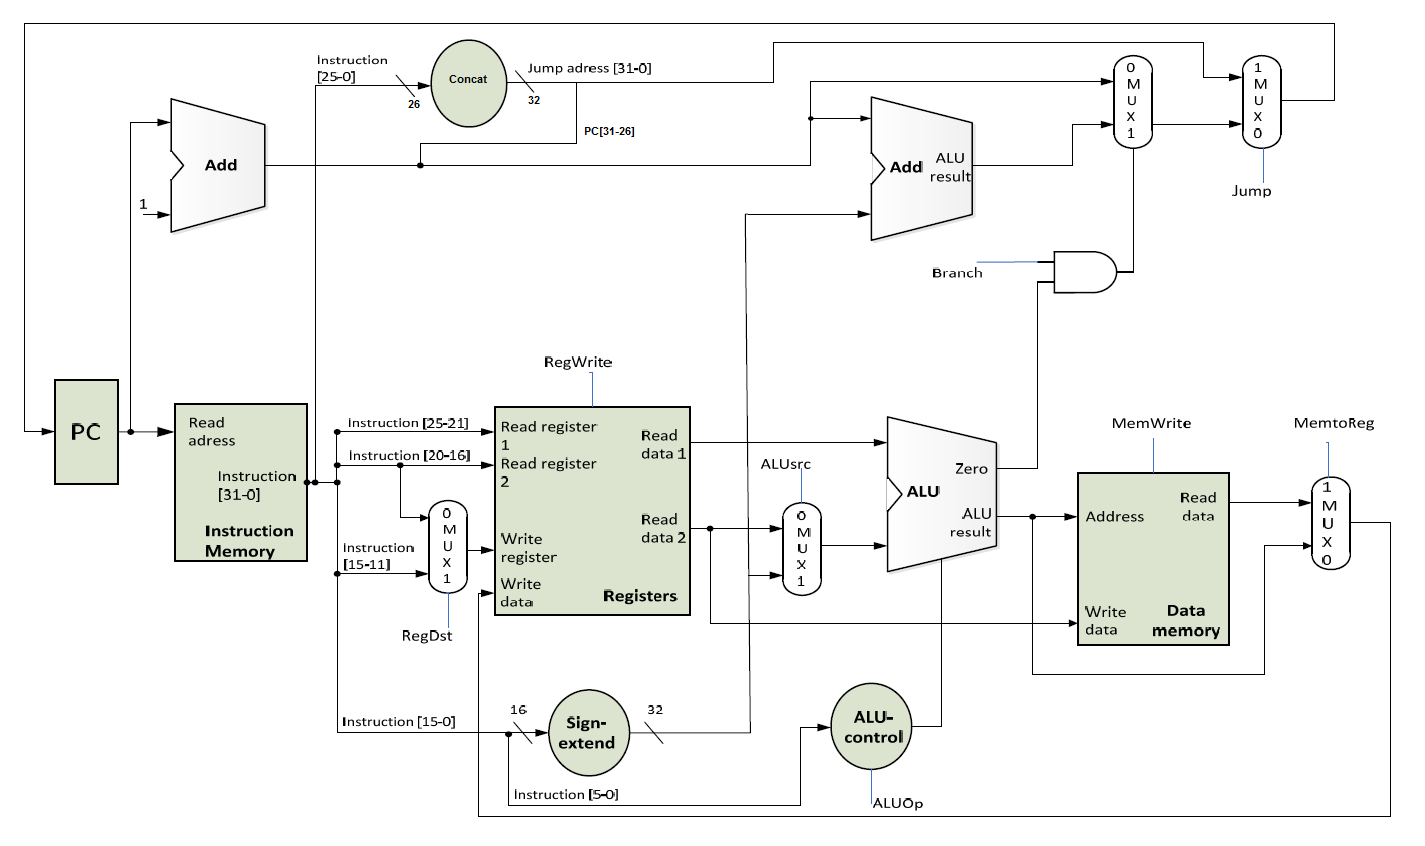
\includegraphics[scale=0.3]{figures/suggestedarchitecture.png}
    \caption{\label{fig:sugarchi}Suggested Architecture \cite[p.115]{lab-compendium}.}
\end{figure}

\section{Suggestions}
It was suggested to use a state machine with the states Fetch, Execute and Stall, where Fetch would retrieve the instruction from memory and Execute would run the instruction. Stall would only be needed in case of data memory access.


\newpage

\part{Solution}

\section{Instruction Set}

The processor implements all required instructions, as shown below:

\begin{itemize}
    \item Several ALU instructions (All working on two registers and storing the result in a third):
        \begin{itemize}
            \item ADD - Addition
            \item SUB - Subtraction
            \item SLT - Test if the first source register is less than second
            \item AND - Bitwise and
            \item OR  - Logical or
        \end{itemize}
    \item BEQ - branch if registers are equal
    \item LW - Load word from memory
    \item SW - Store word to memory
    \item LUI - Store immediate value shifted left 16 bits in a register
    \item J - Jump
\end{itemize}

\section{Architecture}

\begin{figure}[ht]
    \centering
    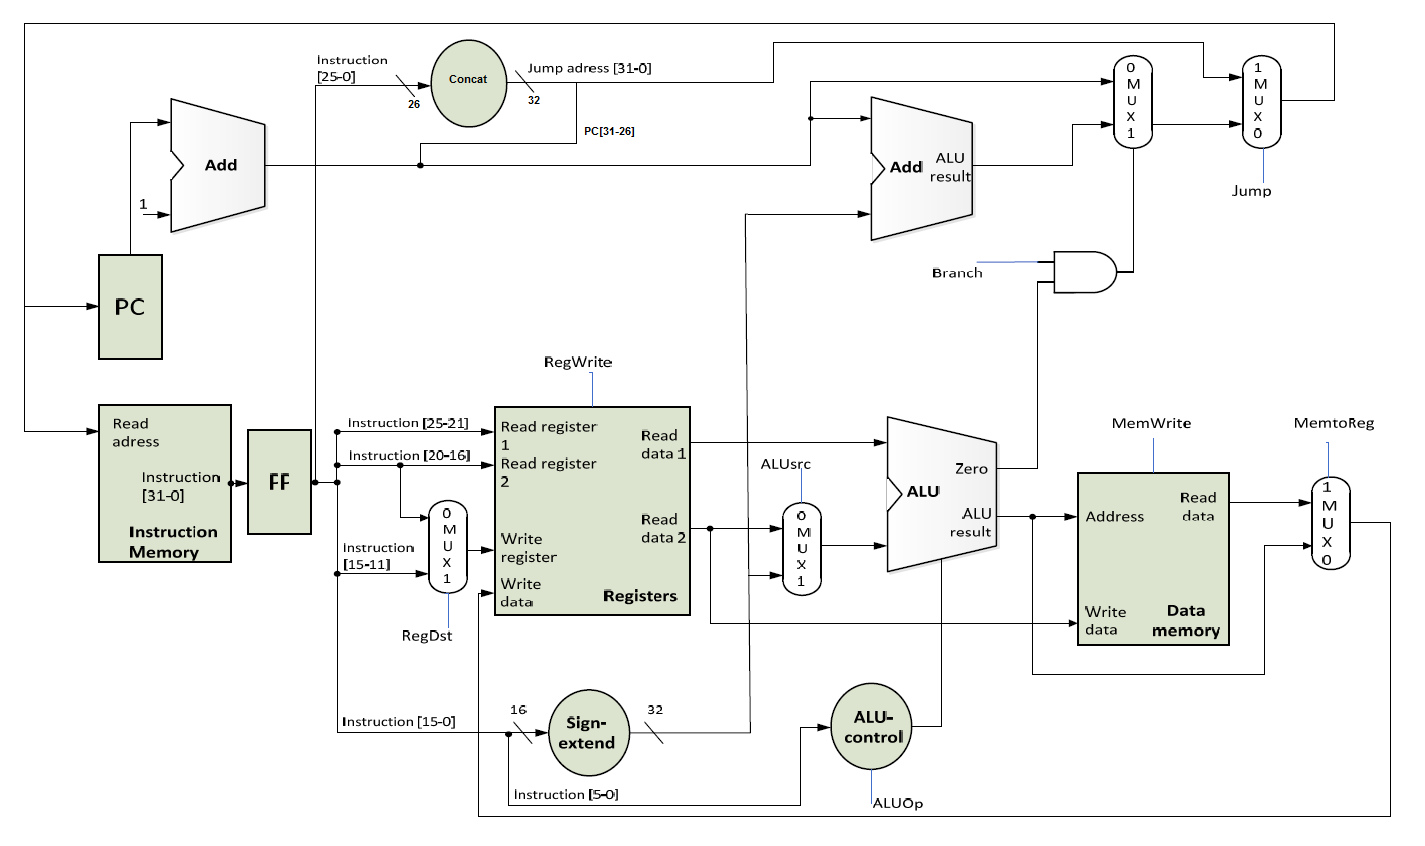
\includegraphics[scale=0.3]{figures/cpu2.png}
    \caption{\label{fig:cpuArchitecture}The implemented CPU architecture.} 
\end{figure}

The CPU architecture closely resembles the suggested one \cite[p.115]{lab-compendium}.
The main difference is that instead of feeding the program counter register into the instruction memory, 
the calculated next program counter is fed into it, and then a flip-flop lets the instruction through at the correct time.

\section{The Control Unit}
\begin{figure}[ht]
    \centering
    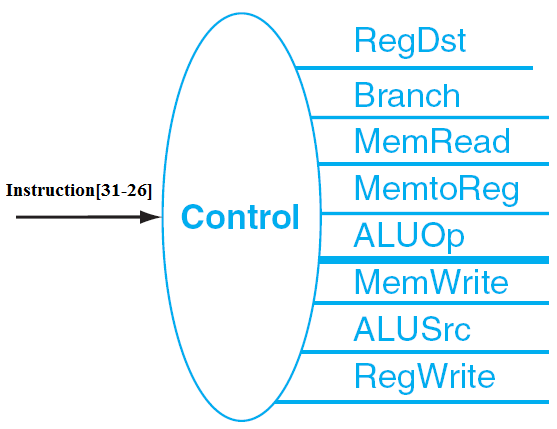
\includegraphics[scale=0.3]{figures/controlunit.png}
    \caption{\label{fig:controlUnit}The control unit.}
\end{figure}

The control unit (CU) was implemented as a state machine, a decoder and a
splitter. On a rising clock edge, it will update the state depending on the
current state. The states, as shown in \ref{fig:stateMachine}, are as follows:

\subsection{Fetch}

The instruction is fetched from the instruction memory and the program counter
is updated before the state is set to execute.

\subsection{Execute}

The CU lets the ALU and other logic do its things before setting the state to
that decided by the decoder, which is normally fetch, but stall in case of load
instructions.

\subsection{Stall}

The CU gives the memory an extra cycle to write the data back to the registers,
before setting the state to fetch.

\subsection{Other}

If the CU finds itself in some other state, something weird has gone wrong.
This is only a sanity check, and should never happen.

\begin{figure}[ht] \centering
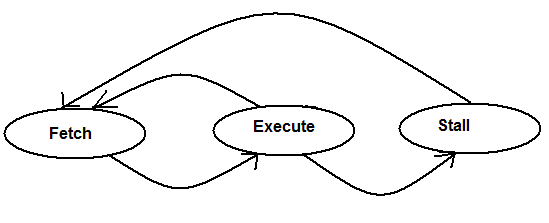
\includegraphics[scale=0.5]{figures/controlunitstatemachine.png}
\caption{\label{fig:stateMachine}The state machine} \end{figure}

\section{Splitter And Decoder}

The splitter simply splits the signal from the instruction memory into its
individual components like opcode, rs, rt, rd and so forth.  The decoder
analyzes the opcode and function signals and enables the correct control signals
and decides the next state.  It is composed of a switch statement with one
condition-block for each opcode.  The R-format has an additional switch
statement to decide the ALU function input.



\newpage

\part{Results}

\section{Simulation}


\newpage

\part{Discussion}

\section{Instruction Set}

While no more instructions than those required were implemented in the processor, it would be a simple matter to implement further instructions by adding more condition-blocks to the case statement of the decoder.

\section{Stall State}

It was suggested to use a stall state for both load and store instructions, but we found that stalls were unnecessary for store instructions, as storing data to the memory only takes one clock cycle, opposed to retrieving data and then writing to registries, which takes two.

\section{Problems}

\subsection{Program Counter}

The program counter has to be updated before the Fetch state in the suggested design. We tried to update it during the Execute state, but this caused some trouble for load instructions, as the destination register and control signals would be changed to that of the next instruction. We therefore decided to add a flip-flop after the instruction memory to control its output. However, this also meant that we had to move the register for the program counter, otherwise it would require two clock cycles to fetch the instruction.

\subsection{Loading the design on to the FPGA}
\label{subsec:uploadproblems}

After successfully generating the programming file, we went on to upload the processor to the FPGA.
AvProg managed to connect to the FPGA board, and upload seemed to going well, it went as far as saying so only to give an error message a second later: \textbf{No ACK from state 12}.
The problem persisted even after increasing AvProg's timeout (as suggested by \cite{avnet-programming-user-manual}, page 40).

It seemed like we were able to connect to the FPGA with host.py and send commands, but we never got any response so we have no idea whether we actually managed to connect.
As the deadline approached by a second every second and we did not manage to come any closer to uploading, we decided it was a better use of our time to improve on what we actually could improve.


\end{document}
